\chapter{Bewijzen van logisch gevolg}\label{ch:bewijzen}
De bewijzen hiervoor waren gegeven door voor de onderhavige proposities de waarheidstabellen op te stellen en te controleren of de zaak klopt. Dit is echter soms erg bewerkelijk. Zo moet er voor het bewijzen van de propositie $((p\rightarrow q)\land(r\rightarrow s))\rightarrow((p\land r)\rightarrow(q\land s))$, met vier verschillende atomen, een waarheidstabel gemaakt worden met maar liefst 16 ($=2^4$) regels. Bovendien zijn sommige proposities tamelijk ingewikkeld, zodat er veel kolommen moeten worden ingevuld.

Soms kunnen we toe met aanzienlijk minder werk\footnote{In wat nu volgt veronderstellen we dat $A$ en $B$ proposities zijn, opgebouwd uit $p, q, r, \ldots$.}. We hoeven bijvoorbeeld voor de controle van de waarheid van $A\rightarrow B$ alleen te kijken naar waarheidswaarden van $p,q,r, \ldots$ waarvoor $A$ waar is, en voor die waarden te controleren of $B$ ook waar is. Immers, volgens de definitie is $A\rightarrow B$ altijd waar als $A$ onwaar is. We formuleren dit principe als volgt:

\begin{quote}
Als $B$ waar is voor alle waarheidswaarden $p, q, r, \ldots$ waarvoor $A$ waar is, dan is $A\rightarrow B$ een tautologie.
\end{quote}
%
Dit principe heet \textit{deductie}. Iets minder precies gezegd luidt dit principe:
\begin{quote}
Als $B$ waar is onder de veronderstelling dat $A$ waar is, dan is $A\rightarrow B$ een tautologie.
\end{quote}
%
Deductie is de methode waarbij een gevolgtrekking wordt gemaakt uit het algemene naar het bijzondere.

De basisstructuur voor het toepassen van het deductieprincipe is: als we een \textit{bewijs} moeten geven dat $P\rightarrow Q$ een tautologie is, beginnen we met een regel `stel dat $P$', en proberen vanuit het gegeven te bewijzen dat $Q$ geldt. Als dat lukt is daarmee het gevraagde bewezen. In zo'n redenering noemen we $P$ de \textit{veronderstelling} (of \textit{premisse}, \textit{aanname} of \textit{hypothese}) en $Q$ de \textit{conclusie} (of het \textit{gevolg}). Hierin kunnen $P$ en $Q$ zelf weer net zulke ingewikkelde proposities zijn als je zelf wilt.

Laten we als voorbeeld bewijzen dat $((p\rightarrow q)\land(r\rightarrow s))\rightarrow((p\land r)\rightarrow(q\land s))$ een tautologie is.

\begin{proof}\mbox{}\\
\begin{tabular}{lll}
(1) & \multicolumn{2}{l}{stel $(p\rightarrow q)\land (r\rightarrow s)$ is waar, dan} \\
(2) & $p\rightarrow q$ is waar  & (volgt uit (1) en definitie \ref{def:conj}) \\
(3) & $r\rightarrow s$ is waar  &(volgt uit (1) en definitie \ref{def:conj}) \\
(4) & \multicolumn{2}{l}{te bewijzen: $(p\land r)\rightarrow(q\land s)$ is waar} \\
& \multicolumn{2}{l}{\begin{tabular}{lll}
(4.1) & $p\land r$ is waar & aanname \\
(4.2) & $p$ is waar $\qquad$& (volgt uit (4.1) en definitie \ref{def:conj}) \\
(4.3) & $r$ is waar & (volgt uit (4.1) en definitie \ref{def:conj}) \\
(4.4) & $q$ is waar &  (volgt uit (4.2) en (2) en modus ponens (\ref{tab:gevolg}).) \\
(4.5) & $s$ is waar &  (volgt uit (4.3) en (3) en modus ponens) \\
(4.6) & $q\land s$ is waar & (volgt uit (4.4) en (4.5) en definitie \ref{def:conj}) \\
\multicolumn{2}{l}{\textsc{einde bewijs} (4)} & (wegens deductie)
\end{tabular}} \\
\multicolumn{2}{l}{\textsc{einde bewijs}} & (wegens deductie)
\end{tabular}\\
\end{proof}
%
Elke regel in het bewijs is zelf weer een bewering die waar is op grond van wat je op dat moment weet. Voor stappen (1)-(3) en (4.1)-(4.6) staat in haakjes aangegeven waarom het geldt. Het \textit{subbewijs} (4.1)-(4.6) is nodig om regel (4) te bewijzen. In de verantwoording mag men refereren aan eerder gemaakte afspraken of stellingen of axioma's, of aan \textit{eerder in het bewijs opgeschreven} proposities. Om deze verwijzing goed aan te kunnen geven zijn de regels genummerd.

Bij de verantwoording van de stappen in een subbewijs mag ook worden gerefereerd aan de eerder in het grote bewijs opgeschreven proposities, met uitzondering van de te bewijzen propositie. Verder mag in het grote bewijs \textit{niet} worden gerefereerd aan proposities in een eerder subbewijs: als je binnen een subbewijs `stel $P$' gezegd hebt, mag je na het afsluiten van het subbewijs niet aannemen dat $P$ nog steeds geldt.


\section{Afleidingsregels}
In het gegeven bewijs hebben we in de motivaties gerefereerd aan de eerder genoemde definities. In het kort hebben we de volgende regels gebruikt:
\begin{enumerate}
\item als $P\land Q$ waar is, dan is $P$ waar;
\item als $P\land Q$ waar is, dan is $Q$ waar;
\item als $P$ en $P\rightarrow Q$ waar zijn, dan is $Q$ waar;
\item als $P$ en $Q$ waar zijn, dan is $P\land Q$ waar.
\end{enumerate}
Dit zijn allemaal regels waarvan iedereen op zijn klompen kan aanvoelen dat het wel klopt, maar toch is het goed en handig om een zo volledig mogelijke lijst op te stellen van zogenaamde \textit{afleidingsregels} die we mogen hanteren. %Een volledige lijst van afleidingsregels voor deductie worden gegeven in sectie \ref{sec:nat:deduc}.

Het toepassen van deductie, met het openen en sluiten van subbewijzen, is een complex en creatief proces, wat voor deze cursus te ver gaat om in zijn geheel te behandelen. Desalniettemin willen we graag bewijzen kunnen leveren, zonder voor de te bewijzen proposities waarheidstabellen te hoeven tekenen. De boommethode is hiervoor een geschikt alternatief.
De \textit{boommethode} is een variant van de zogenaamde \textit{tableaumethode} van de Nederlandse logicus E.W.~Beth. De boommethode is een \textit{semantische} methode, waarmee wordt bedoeld dat deze is gebaseerd op de betekenis van de concepten.

In Figuur \ref{fig:regels} geven we de regels die van toepassing zijn voor de boommethode. In sectie \ref{sec:boom} zullen we uitleggen hoe we deze regels kunnen gebruiken om bewijzen te construeren.

\begin{figure}[ht]
$\begin{array}{|c||c|c||c|c|}
\hline
\neg\text{-regel} & \multicolumn{2}{c||}{\land\text{-regels}} & \multicolumn{2}{c|}{\lor\text{-regels}} \\
\hline\hline
\neg\neg A & A\land B & \neg(A\land B) & A\lor B & \neg(A\lor B) \\
\vdots & \vdots & \vdots & \vdots & \vdots \\
\mathbf{A} & \mathbf{A} & \mathbf{\neg A\lor\neg B} & \text{\huge $\mathbf{\bigwedge}$} & \mathbf{\neg A\land\neg B} \\
 & \mathbf{B} & & \mathbf{A\qquad B} & \\
 \hline
 \multicolumn{5}{c}{}\\
 \hline
 \multicolumn{2}{|c||}{\rightarrow\text{-regels}} & \multicolumn{3}{c|}{\leftrightarrow\text{-regels}} \\
 \hline\hline
 \multicolumn{1}{|c|}{ A\rightarrow B} & \multicolumn{1}{c||}{\neg(A\rightarrow B)} & \multicolumn{1}{c|}{A\leftrightarrow B} & \multicolumn{2}{c|}{\neg(A\leftrightarrow B)} \\
 \multicolumn{1}{|c|}{\vdots} & \multicolumn{1}{c||}{\vdots} & \multicolumn{1}{c|}{\vdots} & \multicolumn{2}{c|}{\vdots} \\
 \multicolumn{1}{|c|}{\mathbf{\neg A\lor B}} & \multicolumn{1}{c||}{\mathbf{A\land\neg B}} & \multicolumn{1}{c|}{\mathbf{A\rightarrow B}} & \multicolumn{2}{c|}{\mathbf{\neg(A\rightarrow B)\lor\neg(B\rightarrow A)}} \\
 \multicolumn{1}{|c|}{} & \multicolumn{1}{c||}{} & \multicolumn{1}{c|}{\mathbf{B\rightarrow A}} & \multicolumn{2}{c|}{} \\
 \hline
\end{array}$
\caption{Afleidings\-regels propositie\-logica}\label{fig:regels}
\end{figure}

De regels in Figuur \ref{fig:regels} dienen van boven naar beneden gelezen te worden. De eerste formule in elke regel duidt de \textit{premisse} aan, terwijl de overige formules, die vet zijn gedrukt, de \textit{conclusies} zijn. Er geldt uiteraard nog steeds dat $A$ en $B$ samengestelde proposities mogen zijn (opgebouwd uit $p,q,r,\ldots$).

De premissen van een regel geeft aan op welke formules men de regel mag toepassen. Wil men bijvoorbeeld de $\neg$-regel toepassen op een zeker formule $F$, dan dient $F$ de formule $\neg\neg A$ te zijn voor een zekere $A$ (opgebouwd uit atomen $p, q, r, \ldots$). Het resultaat van de toepassing van die regel is dan de formule $A$. Het is \textit{niet} toegestaan om een regel toe te passen op subformules van een formule. Zo is de $\neg$-regel \textbf{niet} van toepassing op de formule $\neg\neg A\land B$ omdat hierin $\neg\neg A$ een subformule is. Wel zou men eerst de $\land$-regel kunnen toepassen, met als conclusies $\neg\neg A$ en $B$, om vervolgens $\neg\neg A$ om te zetten in $A$.

\section{Boommethode}\label{sec:boom}
De boommethode wordt gebruikt om vanuit een gegeven verzameling formules te bepalen of andere formules afleidbaar zijn; d.w.z, gegeven een eindige verzameling premissen wordt gekeken of een of andere propositie (de conclusie) vervulbaar danwel onvervulbaar is.% \footnote{ In de klassieke logica is een propositie vervulbaar als er een toekenning, waar of onwaar, bestaat van de atomaire formules in die propositie zodat de propositie waar is. Als er geen toekenning bestaat, dan is de propositie onvervulbaar. Een onvervulbare propositie wordt ook wel een contradictie genoemd. De vervulbaarheid van een formule kan bijvoorbeeld met een waarheidstabel worden gecontroleerd.}. 

\begin{definition}[Vervulbaarheid / onvervulbaar]\mbox{}\\
Een formule heet \textit{vervulbaar} dan en slechts dan als er tenminste \'e\'en toekenning bestaat voor de atomaire proposities in de formule zodat de formule waar wordt. 

Als dat niet het geval is (d.w.z., geen enkele toekenning van waarde aan de atomaire proposities maakt de formule waar), dan heet die propositie \textit{onvervulbaar}.
\end{definition}

In de klassieke logica is een formule vervulbaar als er een toekenning, waar of onwaar, bestaat van de atomaire proposities in die formule zodat de formule waar wordt. Als er geen toekenning bestaat, dan is de formule onvervulbaar. Een onvervulbare formule wordt ook wel een contradictie genoemd. De vervulbaarheid van een formule kan bijvoorbeeld met een waarheidstabel worden gecontroleerd.

\begin{corollary}[Vervulbaar / onvervulbaar]\mbox{}
\begin{enumerate}
\item Tenminste \'e\'en regel van de waarheidstabel van een vervulbare formule bevat een \textit{true}.
\item G\'e\'en van de regels van de waarheidstabel van een onvervulbare formule bevat een \textit{true}.
\item Elke onvervulbare formule is een \textit{contradictie}, en elke contradictie is onvervulbaar.
\item Elke \textit{tautologie} is altijd vervulbaar, maar een formule die vervulbaar is, is tenminste een \textit{contingentie}.
\end{enumerate}
\end{corollary}

Bij toepassing van de boommethode worden de formules uit de verzameling premissen onder elkaar geplaatst en vervolgens met behulp van de regels uit Figuur \ref{fig:regels} afgebroken, totdat er geen enkele regel meer toepasbaar is\footnote{Aangezien het herhaaldelijk opbreken van dezelfde regel geen nieuwe resultaten op gaat leveren, loont het om elke regel die `op' gebruikt is te markeren (bijv. met een `*' of `$\checkmark$'). In deze reader zullen we dit echter achterwege laten.}. Indien de eerste $\lor$-regel wordt toegepast op een formule van de vorm $A\lor B$, ontstaat er een vertakking, waarbij de formule $A$ links, en de formule $B$ rechts onder de vertakking dient te worden geplaatst. Op deze wijze ontstaat er een \textit{boom}, waarvan de bovenste formule de \textit{wortel} van de boom wordt genoemd. Formules onderaan de boom die geen afstammelingen bezitten, noemt men de \textit{bladeren} van de boom. Een \textit{tak} van de boom is een pad dat bij de wortel begint en eindigt bij een blad, zodanig dat hij iedere knoop op dat pad slechts \'e\'en keer wordt gepasseerd.

Als dan iedere tak van de aldus geconstrueerde boom een paar complementaire formules $F$ en $\neg F$ bevat, dan is de oorspronkelijke verzameling van formules onvervulbaar. In dit geval zegt men dat de boom \textit{sluit}. Als er echter een tak bestaat die geen paar complementaire formules bevat, dan is de verzameling premissen w\'el vervulbaar. Zo'n tak, waarvan we zeggen dat ze niet sluit of \textit{open} blijft, bevat dan alle informatie die nodig is om een model voor de verzameling formules te construeren. Een toekenning waarbij alle literals in die tak een waarde 1 krijgen is dan namelijk een model voor de verzameling formules. Indien een propositiesymbool $p$ of zijn ontkenning niet voorkomt in deze tak, dan kan de waarde van dat symbool willekeurig worden gekozen.

\newthought{Om de boommethode te gebruiken} om te bepalen of een logisch gevolg geldt, maken we gebruik van de volgende stelling.
\begin{theorem}[Geldigheid logisch gevolg]\mbox{}\label{th:gevolg}\\
Een logisch gevolg $\Gamma\vdash \varphi$ geldig, dan en slechts dan als de verzameling formules $\Gamma,\neg \varphi$ onvervulbaar is.
\end{theorem}
Dit wil zeggen dat, om af te leiden dat $\varphi$ een logische conclusie is vanuit de verzameling premissen in $\Gamma$, we enkel hoeven aan te tonen dat $\Gamma$ en $\neg \varphi$ samen niet vervulbaar zijn. Herinner dat $\Gamma\vdash \varphi$ zoveel wil zeggen als ``overal waar $\Gamma$ waar is, moet ook $\varphi$ waar zijn'' (zie definitie \ref{def:gevolg}, pagina \pageref{def:gevolg}). Intu\"itief is te zien dat deze stelling geldt omdat $\Gamma, \neg \varphi$ op twee manieren onvervulbaar kan zijn; a) $\Gamma$ zelf is onvervulbaar, maar dan is het niet relevant voor het logisch gevolg (we kijken immers alleen naar die regels waarin alle premissen in $\Gamma$ tezamen waar zijn); of b) $\Gamma$ is vervulbaar, maar in combinatie met $\neg \varphi$ is het onvervulbaar. Dat wil dan zeggen dat voor elke regel van de waarheidstabel waar alle premissen in $\Gamma$ een $T$ bevat, een $F$ staat voor $\neg\varphi$. Maar als dat zo is, wil dat dus zeggen dat diezelfde regels (waarop een $T$ staat bij alle premissen van $\Gamma$) er dus een $T$ zou staan voor $\varphi$; oftewel, $\varphi$ is waar in alle gevallen waarin $\Gamma$ waar is.

Een veel gemaakte denkfout is om te denken dat je logisch gevolg kan aantonen door de \textit{vervulbaarheid} van $\Gamma,\varphi$ te checken, maar dit geeft je helaas geen uitsluitsel over de geldigheid van het logische gevolg. Immers, neem voorbeeld \ref{ex:no:gevolg} (pagina \pageref{ex:no:gevolg}): $p\leftrightarrow q\vdash q$ is geen logisch gevolg (wegens regel 1 van de waarheidstabel hieronder), hoewel $p\leftrightarrow q,q$ wel vervulbaar is (wegens regel 4 van de waarheidstabel hieronder).\\
\begin{tikzpicture}
\matrix (M) [matrix of nodes, column sep=1em] {
    $p$ & $q$ & $p \leftrightarrow q$ & $q$  \\
    0 & 0 & 1 & 0 \\
    0 & 1 & 0 & 1 \\
    1 & 0 & 0 & 0 \\
    1 & 1 & 1 & 1 \\
};
\draw (M-1-1.south west) -- (M-1-4.south east);
\draw (M-1-1.north west) -- (M-5-1.south west) -- (M-5-4.south east -| M-1-4.east) -- (M-1-4.north east);
\draw[hublue,ultra thick] (M-5-3.north west) rectangle (M-5-3.south east);
\draw[hublue,ultra thick] (M-5-4.north west) rectangle (M-5-4.south east);
\draw[hublue,ultra thick] (M-2-3.north west) rectangle (M-2-3.south east);
\draw[hublue,ultra thick] (M-2-4.north west) rectangle (M-2-4.south east);
\node at (2.5,-.85) {\color{green!70!black}{\usym{2714}}};
\node at (2.5,.35) {\color{red}{\large\usym{2718}}};
\end{tikzpicture}

Een volledig bewijs van stelling \ref{th:gevolg} zou te uitvoerig zijn voor deze discussie, maar ze is eenvoudig aan te tonen door het maken van een aantal geschikte waarheidstabellen. We laten dit aan de lezer over.

De boommethode kan nu als volgt worden gebruikt om de geldigheid van een redenering dat een conclusie $F$ volgt uit een verzameling premissen $\Gamma$, geschreven als $\Gamma\vdash F$ door de volgende stappen:
\begin{enumerate}
\item Ga na of de premissen $\Gamma$ samen met de formule $\neg F$ vervulbaar is door een boom te construeren.
\item Sluiten alle takken van de boom doordat deze een paar complementaire formules bevatten, dan is de verzameling niet vervulbaar, hetgeen betekend dat de gegeven redenering logisch geldig is.
\item Is er een tak die open blijft en zijn alle mogelijkheden om regels toe te passen uitgeput, dan is de verzameling vervulbaar en levert de betreffende tak een tegenvoorbeeld.
\end{enumerate}

\begin{example} $p\rightarrow q,q\rightarrow r\vdash p\rightarrow r$\\
We zullen dit aantonen door met behulp van de boommethode te laten zien dat de verzameling formules $p\rightarrow q, q\rightarrow r, \neg(p\rightarrow r)$ onvervulbaar is. De boom hiervan is hieronder weergegeven. Alle takken van deze boom sluiten (aangegeven door $\mathbf{X}(m,n)$, hetgeen betekent dat de betreffende tak sluit op de formules met nummers $m$ en $n$. Omdat alle takken sluiten, kunnen we concluderen dat de verzameling $p\rightarrow q,q\rightarrow r, \neg(p\rightarrow r)$ onvervulbaar is, wat aanduidt dat $p\rightarrow q,q\rightarrow r\vdash p\rightarrow r$.
\begin{center}
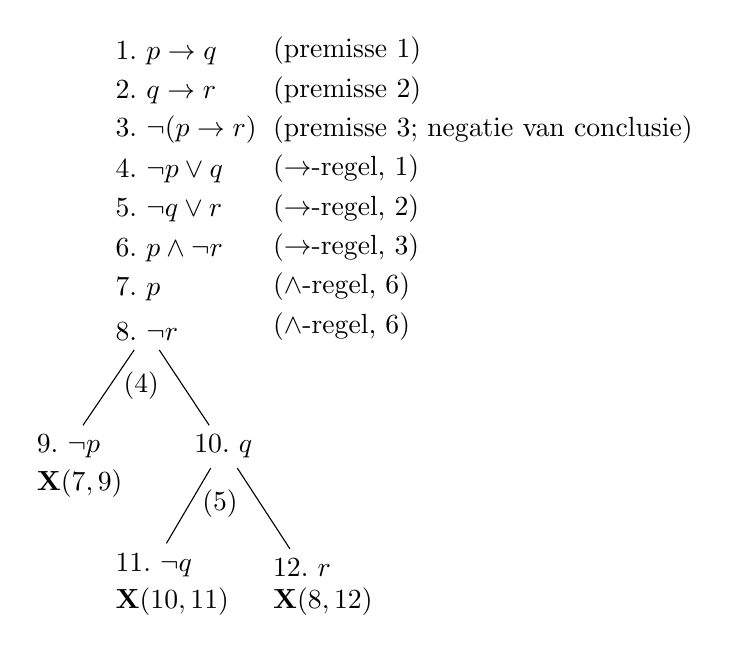
\begin{tikzpicture}[anchor=south west]
\node at (2,6) {$1.\ p\rightarrow q$}; \node at (4,6) {(premisse 1)};
\node at (2,5.5) {$2.\  q\rightarrow r$}; \node at (4,5.5) {(premisse 2)};
\node at (2,5) {$3.\  \neg(p\rightarrow r)$}; \node at (4,5) {(premisse 3; negatie van conclusie)};
\node at (2,4.5) {$4.\  \neg p\lor q$}; \node at (4,4.5) {($\rightarrow$-regel, 1)};
\node at (2,4) {$5.\  \neg q\lor r$}; \node at (4,4) {($\rightarrow$-regel, 2)};
\node at (2,3.5) {$6.\  p\land\neg r$}; \node at (4,3.5) {($\rightarrow$-regel, 3)};
\node at (2,3) {$7.\  p$}; \node at (4,3) {($\land$-regel, 6)};
\node at (2,2.5) (pre) {$8.\  \neg r$}; \node at (4,2.5) {($\land$-regel, 6)};
\node at (1,1) (p1) {$9.\  \neg p$}; \node at (1,0.5) {$\mathbf{X}(7,9)$};
\node at (3,1) (p2) {$10.\  q$};
\draw (p1) -- (pre) -- (p2);
\node at (2.1, 1.75) {$(4)$};
\node at (2,-.5) (p3) {$11.\  \neg q$}; \node at (4,-.5) (p4) {$12.\  r$};
\node at (2,-1) {$\mathbf{X}(10,11)$}; \node at (4,-1) {$\mathbf{X}(8,12)$};
\node at (3.1,0.25) {$(5)$};
\draw (p3) -- (p2) -- (p4);
\end{tikzpicture}
\end{center}
\end{example}

Merk op dat het aantonen dat een formule een contradictie is nu eenvoudig te doen is door het maken van een boom voor de formule zelf (immers, een sluitende boom geeft onvervulbaarheid aan, en contradicties zijn onvervulbaar). Voor het aantonen dat een formule een tautologie is, is een boom voor de negatie van de formule benodigd (immers, de negatie van een tautologie is een contradictie). Om te bewijzen dat iets een formule een contingentie is, zijn helaas wat meer stappen benodigd. Immers dient men dan aan te tonen dat zowel de boom voor de oorspronkelijke formule en de boom voor de negatie van de formule \textit{niet} sluiten\footnote{Als slechts \'e\'en van beide niet sluitende bomen wordt gemaakt, wordt er feitelijk alleen maar aangetoond dat de formule $\varphi$ geen contradictie is (aangetoond door niet sluitende boom voor $\varphi$) \'of dat $\varphi$ geen tautologie is (aangetoond door niet sluitende boom voor $\neg\varphi$).}.


\begin{example} \textit{niet} $\vdash (p\rightarrow q)\rightarrow(q\rightarrow p)$\\
We laten zien hoe met behulp van de boommethode een tegenvoorbeeld kan worden verkregen voor de uitspraak $\vdash (p\rightarrow q)\rightarrow(q\rightarrow p)$ (wat dus zoveel wil zeggen als dat $(p\rightarrow q)\rightarrow(q\rightarrow p)$ g\'e\'en tautologie is). De boom hieronder laat zien dat de verzameling $\neg(p\rightarrow q)\rightarrow(q\rightarrow p))$ vervulbaar is. Geen van de takken van de boom sluit. Een tegenvoorbeeld is bijvoorbeeld te lezen in de linkertak: maak $p$ onwaar en $q$ waar. Hiermee is bewezen dat $\vdash (p\rightarrow q)\rightarrow(q\rightarrow p)$ \textit{niet} geldt!
\begin{center}
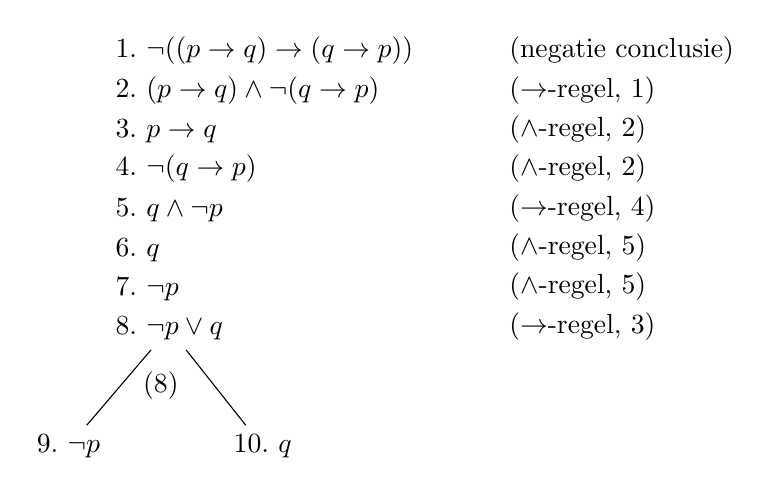
\begin{tikzpicture}[anchor=south west]
\node at (2,6) {$1.\ \neg((p\rightarrow q)\rightarrow(q\rightarrow p))$}; \node at (7,6) {(negatie conclusie)};
\node at (2,5.5) {$2.\ (p\rightarrow q)\land\neg(q\rightarrow p)$}; \node at (7,5.5) {($\rightarrow$-regel, 1)};
\node at (2,5) {$3.\  p\rightarrow q$}; \node at (7,5) {($\land$-regel, 2)};
\node at (2,4.5) {$4.\  \neg(q\rightarrow p)$}; \node at (7,4.5) {($\land$-regel, 2)};
\node at (2,4) {$5.\  q\land\neg p$}; \node at (7,4) {($\rightarrow$-regel, 4)};
\node at (2,3.5) {$6.\  q$}; \node at (7,3.5) {($\land$-regel, 5)};
\node at (2,3) {$7.\  \neg p$}; \node at (7,3) {($\land$-regel, 5)};
\node at (2,2.5) (p1) {$8.\  \neg p\lor q$}; \node at (7,2.5) {($\rightarrow$-regel, 3)};
\node at (1,1) (p2) {$9.\  \neg p$}; \node at (3.5,1) (p3) {$10.\  q$};
\draw (p2) -- (p1) -- (p3);
\node at (2.35, 1.75) {$(8)$};
\end{tikzpicture}
\end{center}
\end{example}

\subsection{Opgaven}
Om de techniek van bewijzen te oefenen, mogen in de volgende opgaven geen waarheidstabellen, gelijkheidswaarheden of tautologi\"en worden gebruikt. Je mag alleen gebruik maken van de in dit hoofdstuk gegeven boommethode.

\begin{exercise}
Bewijs met de boommethode dat:
\begin{enumerate}[label=\textit{\alph*.}]
\item $p\vdash p$
\item $p\wedge q\vdash q$
\item $p\rightarrow q\vdash \neg p\vee q$
\item $\neg p\vdash p\rightarrow q$
\item $\neg(p\vee q)\vdash p\rightarrow q$
\end{enumerate}
\end{exercise}
\begin{exercise} Ga voor elk van de onderstaande beweringen na of dat deze juist danwel onjuist is. Geef in het eerste geval een bewijs met behulp van de boommethode. Construeer in het tweede geval een \textit{tegenvoorbeeld}.
\begin{enumerate}[label=\textit{\alph*.}]
\item $p\rightarrow q$ is een tautologie (d.w.z. $\vdash p\rightarrow q$).
\item $p\rightarrow p$ is een tautologie (d.w.z. $\vdash p\rightarrow p$).
\item $p\leftrightarrow p$ is een tautologie (d.w.z. $\vdash p\leftrightarrow p$).
\item $p\wedge\neg q$ is een contradictie (d.w.z $\not\vdash p\wedge\neg q$ ofwel $\vdash\neg(p\wedge\neg q)$).
\item $p\wedge\neg p$ is een contradictie (d.w.z. $\not\vdash p\wedge\neg p$).
\item $p\leftrightarrow\neg p$ is een contradictie (d.w.z. $\not\vdash p\leftrightarrow\neg p$).
\end{enumerate}
\end{exercise}
\begin{exercise} Bewijs met de boommethode dat:
\begin{enumerate}[label=\textit{\alph*.}]
\item $p, (p\land\neg q)\rightarrow r, \neg (p\land r)\vdash q$.
\item $\neg p\leftrightarrow(q\lor r), p\land r\vdash\neg q$.
\item $p\leftrightarrow(\neg q\lor\neg r), \neg(\neg p\rightarrow r)\vdash \neg q$.
\item $p\rightarrow((q\rightarrow r)\rightarrow s), \neg(p\rightarrow s)\vdash\neg(q\rightarrow r)$.
\item $(p\land q)\rightarrow r,\neg p\lor(p\rightarrow q)\vdash p\rightarrow r$.
\item $(p\rightarrow\neg r)\lor(p\rightarrow q), r\rightarrow p\vdash r\rightarrow q$.
\end{enumerate}
\end{exercise}
\begin{exercise}Ga voor elk van de onderstaande beweringen na of deze juist dan wel onjuist is. Geef in het eerste geval een bewijs met behulp van de boommethode. Construeer in het tweede geval een \textit{tegenvoorbeeld}.
\begin{enumerate}[label=\textit{\alph*.}]
\item $p\rightarrow q,\neg r\rightarrow q\vdash p\rightarrow r$.
\item $\vdash ((p\lor(p\rightarrow q))\rightarrow q)\rightarrow q$.
\item $(p\land q)\rightarrow s, \neg(s\rightarrow t), q\lor t\vdash \neg p$.
\item $\neg p\rightarrow p\vdash p$.
\item $\vdash (p\lor q)\rightarrow (p\land q)$.
\item $\neg p,p\vdash q$.
\end{enumerate}
\end{exercise}
\begin{exercise} Vertaal de volgende redeneringen naar \textit{propositielogica} en ga met behulp van de boommethode na of deze logisch geldig zijn of niet. Produceer in het laatste geval ook een tegenvoorbeeld.
\begin{enumerate}[label=\textit{\alph*.}]
\item \textit{Als Tom nuchter is, dan handelt hij rationeel maar hij is dan wel oninteressant.}\\
\textit{Als hij beleefd en oninteressant is, dan vindt Sylvia hem niet aardig.}\\
\textit{Dus, als Tom nuchter en beleefd is, dan vindt Sylvia hem niet aardig.}
\item\textit{Als Anton lid wordt van de Nederlandse Vereniging van Terraszitters, dan worden Bob en Cees dat ook.}\\
\textit{Als Anton of Bob lid wordt, dan zal David zijn lidmaatschap opzeggen.}\\
\textit{Dus zal David zijn lidmaatschap opzeggen, ongeacht of Cees nou lid wordt of niet.}
\item\textit{Je kunt Hans geloven als je Bert kunt geloven, en omgekeerd.}\\
\textit{Als je noch Hans, noch Bert kunt geloven, dan kun je ook Greetje niet geloven.}\\
\textit{Je kunt Greetje geloven.}\\
\textit{Dus je kunt Bert geloven.}
\end{enumerate}

\end{exercise}

%\section{Natuurlijke deductie *}\label{sec:nat:deduc}
%\begin{remark}
%De stof in deze sectie behoort niet tot de basisstof van het vak en zal niet getentamineerd worden. Ze is enkel toegevoegd voor ge\"interesseerde studenten die \textit{verder} willen dan de gemiddelde student.
%\end{remark}
%
%Eerder, in sectie \ref{sec:boom}, hebben we wat spelregels ge\"introduceerd voor het uitvoeren van deductie. In deze sectie zullen we daarop verder bouwen en alle regels introduceren. We zullen ook elke regel een naam geven, zodat we in motivaties in bewijzen alleen die naam hoeven te noemen in plaats van de hele regel zelf op te schrijven.
%
%Voor afleidingsregels gebruiken we de volgende notatie.
%$$A, B,\ldots \vdash C, D,\ldots$$
%Dit dient gelezen te worden als: als \textit{elk} van de proposities \textit{links} van $\vdash$ waar is of verondersteld wordt waar te zijn, dan mag de waarheid van elke propositie \textit{rechts} van de $\vdash$ geconcludeerd worden.
%
%Een andere veel gebruikte notatie voor hetzelfde doel is de conclusiestreep
%$$\frac{A,B,\ldots}{C,D,\ldots}\text{ betekent hetzelfde als }A,B,\ldots\vdash C,D,\ldots$$
%De afleidingsregels die gelden voor natuurlijke deductie zijn de volgende.
%\begin{center}\begin{tabular}{|lc|}
%\hline\\[-1em]
%& (sub)bewijs beginnend met \\ 
%\textit{deductie} & $A$ (veronderstelling) en eindigend met $B$\\
%& $\qquad \vdash A\rightarrow B$\\[0.5em]
%\hline\\[-1em]
%\textit{modus ponens} & $A, A\rightarrow B\vdash B$\\[0.5em]
%\hline\\[-1em]
%\textit{introductie-$\land$} & $A, B\vdash A\land B$\\[0.5em]
%\hline\\[-1em]
%\textit{eliminatie-$\land$} & $A\land B\vdash A, B$\\[0.5em]
%\hline\\[-1em]
%\textit{introductie-$\lor$} & $A\vdash A\lor B, B\lor A$\\[0.5em]
%\hline\\[-1em]
%\textit{eliminatie-$\lor$} & $A\lor B, A\rightarrow C, B\rightarrow C\vdash C$\\[0.5em]
%\hline\\[-1em]
%\textit{introductie-$\leftrightarrow$} & $A\rightarrow B, B\rightarrow A\vdash A\leftrightarrow B$\\[0.5em]
%\hline\\[-1em]
%\textit{eliminatie-$\leftrightarrow$} & $A\leftrightarrow B\vdash A\rightarrow B, B\rightarrow A$\\[0.5em]
%\hline\\[-1em]
%\textit{introductie-$\neg$} & $B\rightarrow\bot\vdash\neg B$\\[0.5em]
%\hline\\[-1em]
%\textit{introductie-$\bot$} & $A,\neg A\vdash\bot$\\[0.5em]
%\hline\\[-1em]
%\textit{eliminatie-$\bot$} & $\bot\vdash A$\\[0.5em]
%\hline\\[-1em]
%\textit{gevalsonderscheid} & $\vdash A\lor\neg A$\\[0.5em]
%\hline
%\end{tabular}
%\end{center}
%
%Op deze wijze hebben we voor elk van de connectieven een introductieregel waarmee een propositie \textit{bewezen} kan worden waarin dat connectief voorkomt, en voor elk van de binaire connectieven een eliminatie regel waarmee een propositie \textit{gebruikt} kan worden waarin dat connectief voorkomt. Hierin speelt deductie de rol van \textit{introductie-$\rightarrow$} en modus ponens de rol van \textit{eliminatie-$\rightarrow$}. Om historische redenen gebruiken we echter de begrippen deductie en modus ponens.
%
%In plaats van de regel \textit{gevalsonderscheid} hadden we ook een regel $\vdash\top$ kunnen invoeren onder de naam \textit{introductie-$\top$} en een regel $\top\vdash A\lor\neg A$ onder de naam \textit{eliminatie-$\top$}. Deze regels worden echter voornamelijk in combinatie gebruikt, en daarom hebben we de combinatie gelijk maar als regel ingevoerd. Zo kan hij vaak handig worden gebruikt, in het bijzonder om eliminatie-$\lor$ te kunnen toepassen: als we $A\rightarrow C$ en $\neg A\rightarrow C$ hebben afgeleid, kunnen we met deze regel en eliminatie-$\lor$ concluderen dat dan ook $C$ geldt. Hiermee is $C$ in feite bewezen door een gevalsonderscheid tussen $A$ en $\neg A$ te maken. Immers, in de klassieke logica zijn er maar twee gevallen te onderscheiden wat betreft een variabele $A$; deze is waar, of deze is niet waar. Als uit beide gevallen blijkt dat je $C$ kan afleiden, dan geldt dat dus altijd (alle gevallen zijn gedekt).
%
%Er zijn nog wel meer regels te verzinnen. We beperken ons echter tot de hier gegeven lijst.
%
%De systematiek van de lijst kun je opvatten als hulpmiddel om een bewijs te vinden. Zo word je gedwongen om de bijbehorende introductieregel toe te passen als je de geldigheid van een bepaalde propositie wilt bewijzen. Preciezer gezegd:
%\begin{itemize}
%\item Als je de geldigheid van $A\rightarrow B$ wilt bewijzen, moet je deductie toepassen, oftewel je begint met $A$ te stellen en je moet vervolgens $B$ bewijzen.
%\item Als je de geldigheid van $A\land B$ wilt bewijzen, moet je introductie-$\land$ toepassen, oftewel je moet zowel $A$ als $B$ bewijzen.
%\item Als je de geldigheid van $A\lor B$ wilt bewijzen, moet je introductie-$\lor$ toepassen, oftewel je moet $A$ bewijzen of $B$ bewijzen.
%\item Als je de geldigheid van $\neg A$ wilt bewijzen, moet je introductie-$\neg$ toepassen, oftewel je moet $A\rightarrow\bot$ bewijzen, en dat moet je weer met deductie doen. In feite geef je hiermee een \textit{bewijs uit het ongerijmde}.
%\end{itemize}
%
%Als voorbeeld bewijzen we, uitsluitend gebruik makend van deze afleidingsregels dat $(p\rightarrow q)\rightarrow(\neg p\lor q)$ een tautologie is.
%\begin{example}  $(p\rightarrow q)\rightarrow(\neg p\lor q)$ is een tautologie.
%\begin{proof}\mbox{}\\
%\begin{tabular}{lll}
%(1) & $p\rightarrow q$ & (veronderstelling) \\
%(2) & $p\lor\neg p$ & (gevalsonderscheiding) \\
%(3) & \multicolumn{2}{l}{te bewijzen: $p\rightarrow(\neg p\lor q)$}\\
%& \multicolumn{2}{l}{\begin{tabular}{lll}
%  \multicolumn{3}{l}{\textsc{bewijs} van (3):}\\
%  (3.1) & $p$ & (veronderstelling) \\
%  (3.2) & $q$ & (modus ponens: 1, 3.2) \\
%  (3.3) & $\neg p\lor q$ & (intr.-$\lor$: 3.2) \\
%  \multicolumn{2}{l}{\textsc{einde bewijs (3)}} & (deductie)
%\end{tabular}
%}\\
%(4) & \multicolumn{2}{l}{te bewijzen $(\neg p\rightarrow (\neg p\lor q)$}\\
%& \multicolumn{2}{l}{\begin{tabular}{lll}
%  \multicolumn{3}{l}{\textsc{bewijs} van (4):}\\
%  (4.1) & $\neg p$ & (veronderstelling) \\
%  (4.2) & $\neg p\lor q$ & (intr.-$\lor$, 4.1) \\
%  \multicolumn{2}{l}{\textsc{bewijs} van (4)} & (deductie)
%\end{tabular}} \\
%(5) & $\neg p\lor q$ & (elim.-$\lor$: 2, 3, 4) \\
%\multicolumn{2}{l}{\textsc{einde bewijs}} & (deductie)
%\end{tabular}\\
%\end{proof}
%\end{example}
%
%Het is geenszins de bedoeling om een keurslijf van exacte, doch cryptisch opgeschreven bewijzen op te dringen. Integendeel, een in goed Nederlands opgeschreven heldere redenering heeft het grote voordeel dat iedereen het kan volgen. Vaak echter schiet het gewone taalgebruik te kort om een argumentatie in weinig woorden waterdicht te maken. Juist in die gevallen is een strak systeem van groot nut. Wel geldt uiteraard bij alle bewijzen dat ze moeten voldoen aan de hier gegeven spelregels, ook als de verschillende beweringen niet expliciet genummerd zijn. De hier gegeven spelregels zijn niet gegeven om het je moeilijk te maken, maar zijn een weerslag van de consensus over wat correcte en geldige redeneringen zijn, en hopen juist een hulpmiddel te zijn om dergelijke redeneringen gestructureerd te kunnen krijgen.
%
%In de praktijk zal men veelal conclusies trekken, zonder de verantwoording tot in de allerkleinste details op te schrijven. Men geeft dan alleen de grote lijnen weer. Op zich is dat niet zo erg, het hoort bij de ontwikkeling tot beoefenaar van een vak. Naarmate de ontwikkeling vordert worden steeds complexere combinaties tot een geheel. Hierin schuilen uiteraard wel grotere gevaren voor vergissingen! Probeer nooit een bewijs zo ``uit te dunnen'' dat je zelf na een paar dagen moeite hebt om te zien ``hoe het ook weer zat''.
%
%\subsection{Opgaven}
%Om de techniek van deductie te oefenen, mogen in de volgende opgaven geen waarheidstabellen, gelijkheidswaarheden, tautologi\"en of boommethode worden gebruikt. Je mag alleen gebruik maken van de in deze sectie ge\"introduceerde afleidingsregels van deductie.
%
%\begin{exercise}
%Bewijs dat $(p\rightarrow q)\rightarrow((p\land r)\rightarrow(q\land r))$ een tautologie is.
%\end{exercise}
%\begin{exercise}
%Bewijs dat $((p\rightarrow q)\land(q\rightarrow r))\rightarrow(p\rightarrow r)$ een tautologie is.
%\end{exercise}
%\begin{exercise}
%Bewijs dat $((p\rightarrow q)\land(r\rightarrow s)\land p\land r)\rightarrow(q\land s))$ een tautologie is.
%\end{exercise}
%\begin{exercise}
%Bewijs dat $((p\rightarrow q)\land(p\rightarrow\neg q))\rightarrow\neg p$ een tautologie is.
%\end{exercise}
%\begin{exercise}
%Bewijs dat $\neg p\rightarrow(p\rightarrow q)$ een tautologie is.
%\end{exercise}
%\begin{exercise}
%Bewijs dat $(p\rightarrow q)\rightarrow(\neg q\rightarrow\neg p)$ een tautologie is.
%\end{exercise}
%\begin{exercise}
%Bewijs dat $(\neg p\leftrightarrow q)\rightarrow\neg(p\leftrightarrow q)$ een tautologie is.
%\end{exercise}
